\usetikzlibrary{automata, positioning, arrows, calc}
\tikzset{
	->,  % makes the edges directed
	>=stealth, % makes the arrow heads bold
	shorten >=2pt, shorten <=2pt, % shorten the arrow
	node distance=2cm, % specifies the minimum distance between two nodes. Change if n
	every state/.style={draw=blue!55,very thick,fill=blue!13}, % sets the properties for each ’state’ n
	initial text=$ $, % sets the text that appears on the start arrow
}

\chapter{graficos}
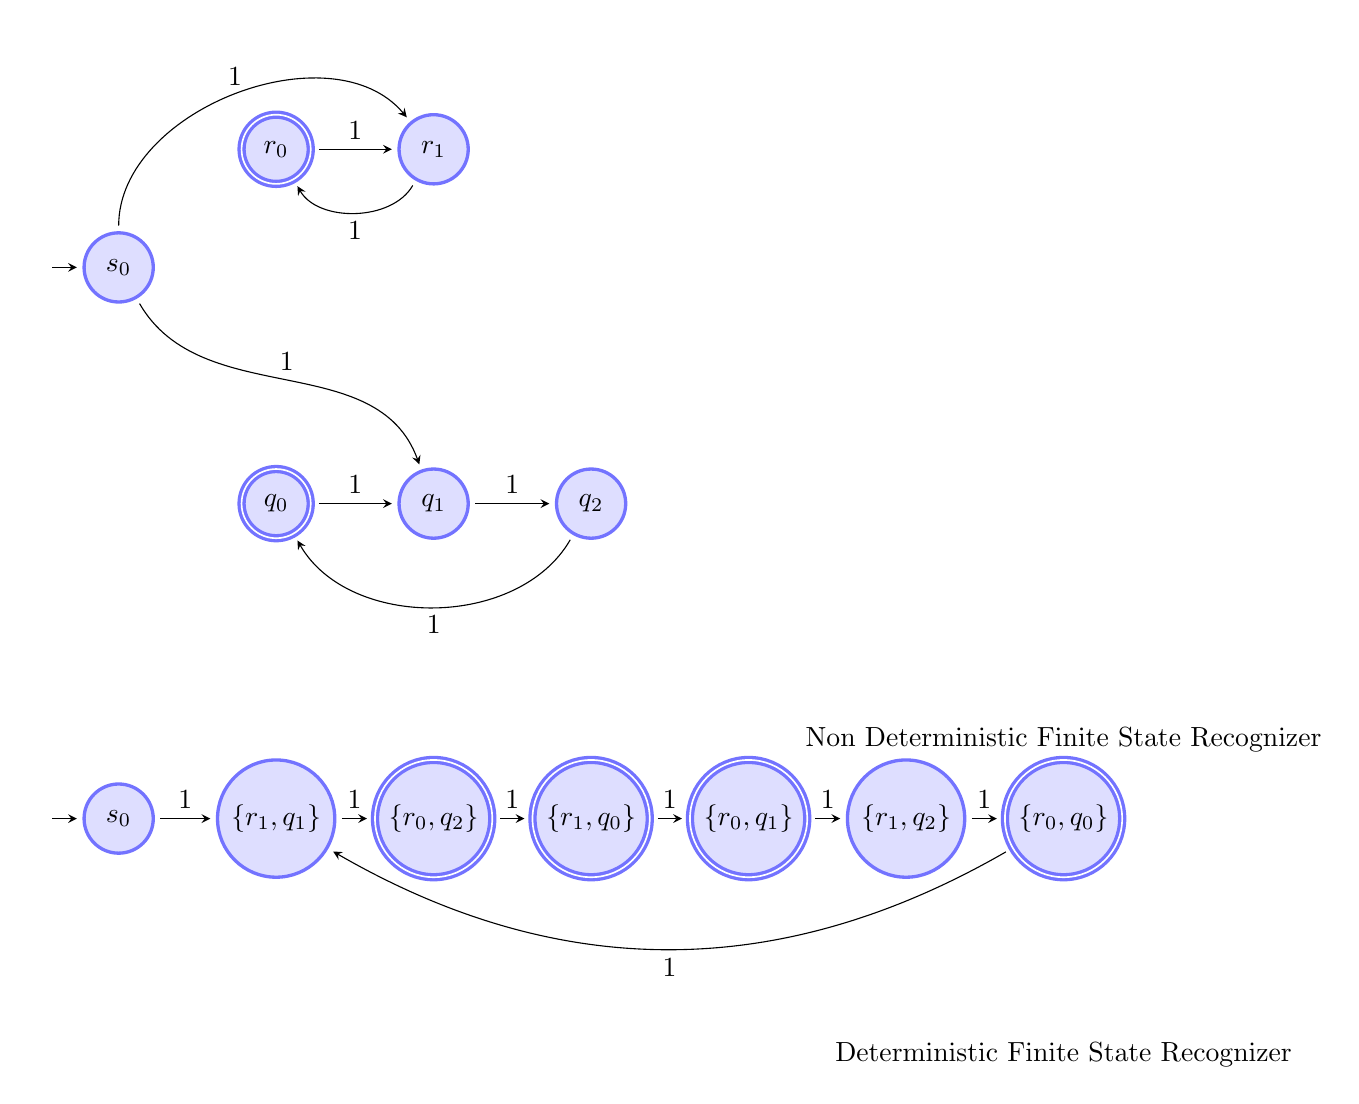
\begin{tikzpicture}
	
	% FSM
	\node[state, initial] (s0) {$s_0$};
	\node[state, right of=s0] (r1q1) {$\{r_1,q_1\}$};
	\node[state, accepting, right of=r1q1] (r0q2) {$\{r_0,q_2\}$};
	\node[state, accepting, right of=r0q2] (r1q0) {$\{r_1,q_0\}$};
	\node[state, accepting, right of=r1q0] (r0q1) {$\{r_0,q_1\}$};
	\node[state, right of=r0q1] (r1q2) {$\{r_1,q_2\}$};		
	\node[state, accepting, right of=r1q2] (r0q0) {$\{r_0,q_0\}$};		
	
	\draw   (s0) edge[above] node{$1$} (r1q1)
	(r1q1) edge[above] node{$1$} (r0q2)
	(r0q2) edge[above] node{$1$} (r1q0)
	(r1q0) edge[above] node{$1$} (r0q1)
	(r0q1) edge[above] node{$1$} (r1q2)
	(r1q2) edge[above] node{$1$} (r0q0)
	(r0q0) edge[bend left, below] node{$1$} (r1q1);
	
	% NDFSM
	\node[state, initial, above of=s0, yshift=+5cm] (s0) {$s_0$};
	\node[state, accepting, right of=s0, yshift=1.5cm] (r0) {$r_0$};
	\node[state, right of=r0] (r1) {$r_1$};
	\node[state, accepting, right of=s0, yshift=-3cm] (q0) {$q_0$};
	\node[state, right of=q0] (q1) {$q_1$};
	\node[state, right of=q1] (q2) {$q_2$};
	
	\draw   (s0) edge[above, out=90, in=130] node{$1$} (r1)
	(r0) edge[above] node{$1$} (r1)
	(r1) edge[below, out=240, in=-60] node{$1$} (r0)
	(s0) edge[above, out=-60, in=110] node{$1$} (q1)
	(q1) edge[above] node{$1$} (q2)
	(q2) edge[below, out=240, in=-60] node{$1$} (q0)
	(q0) edge[above] node{$1$} (q1)
	;
	
	% Text
	\node[yshift=-6cm] at (r0q0|-s0) {Non Deterministic Finite State Recognizer};
	\node[yshift=-3cm] at (r0q0) {Deterministic Finite State Recognizer};
	
	
\end{tikzpicture}